\chapter{Theoretical Background}
\label{chapter:background}
\begin{music}
    \parindent10mm \instrumentnumber{1} \setstaffs1{1} 
    \generalmeter{\meterfrac34} \generalsignature{-1}
    \startextract
		\notes  \en
    \zendextract
\end{music}
\epigraph{\textit{the passion of friendship will soon blossom into a righteous power}}{Bolero of Fire --- Ocarina of Time}

% Convolutional neural networks trained on large databases \cite{mnist2012,imagenet2009} have shaped machine learning research over the past couple of decades. Today they serve as canonical learning material in courses and are often used as initial \textit{vanilla} approaches for data exploration and classification tasks and before creating more bespoke machine learning pipelines. The widespread success of much models created an expectation in the research community that with sufficient data and computational power provided by one of the reigning consumer internet businesses, a data-driven black-box model can be created for any application ranging from quantum mechanics to economics. Convolutional architectures together with language models eventually inspired recurrent architectures and attention models where are the key ingredients in the creation of \textit{Alpha Fold} \cite{Jumper2021HighlyAlphaFold} that takes a substantial step towards solving the protein-folding problem. Biotechnology researchers are eager to apply these methods but face the following obstacles

% \begin{itemize}
%     \item \textbf{Insufficient data} due to strategic experimental designs 
%     \item \textbf{Low extrapolation accuracy} for black box-models
% \end{itemize}

This Chapter lays out a background bifurcation theory and machine learning methods relevant to cell biology and flow cytometry. We establish the connection between the concept of phenotypes and bifurcations in Section \ref{section:phenotypes-with-bifurcations} and lay out assumptions and definitions that are used throughout other chapters. Section \ref{section:applications-cell-biology} follows up with concrete applications of differential equations in cell biology and will prepare the reader for the incorporated synthetic biology publication in Chapter \ref{chapter:double-exclusive}.

The problem of inferring phenotypes from data is defined in Section \ref{section:phenotype-inference} with a survey relevant machine learning methods. This section discusses the pre-processing techniques to extract bifurcations from raw data, as has been done in Chapter \ref{chapter:double-exclusive}, and used as a starting point in the incorporated machine learning publication in Chapter \ref{chapter:inference}. Section \ref{section:applications-flow-cytometry} gives the reader a background in flow cytometry and how the machine learning methods discussed in previous sections are used by immunologists to identify immune cell phenotypes. This section lays the foundations for the interactive exploration tool presented in Chapter \ref{chapter:exploring}.

\section{Describing Phenotypes with Bifurcations}
\label{section:phenotypes-with-bifurcations}

%Bringing in the definition here is too early. Too abrupt.
%Historical context of how the word emerged and how it is used in biological contexts
A phenotype is a qualitative state or behaviour of an organism that can be described by several quantitative features. Before considering the additional complexity that comes with biology, let us first consider a simple everyday metaphor: light bulbs. Light bulbs come in various combinations of quantitative features $\theta$ which could be its shape, colour, materials and circuit design. The purpose of a light bulb is to fulfil a single function: increase in brightness as a function of voltage $p$, pushing the qualitative state of the bulb from \emph{off} to \emph{on}. Changes to bulb shape affect neither its function nor its states. Changes in color affect the quality of the \emph{on} state but not the \emph{off} state. Changes to circuit design and materials may change or even break the bulb's function. Fluorescent bulbs, for example, only have two possible brightness states in response to changes in voltage $p$, while incandescent bulbs have a continuous brightness response.
\\
\begin{Figure}
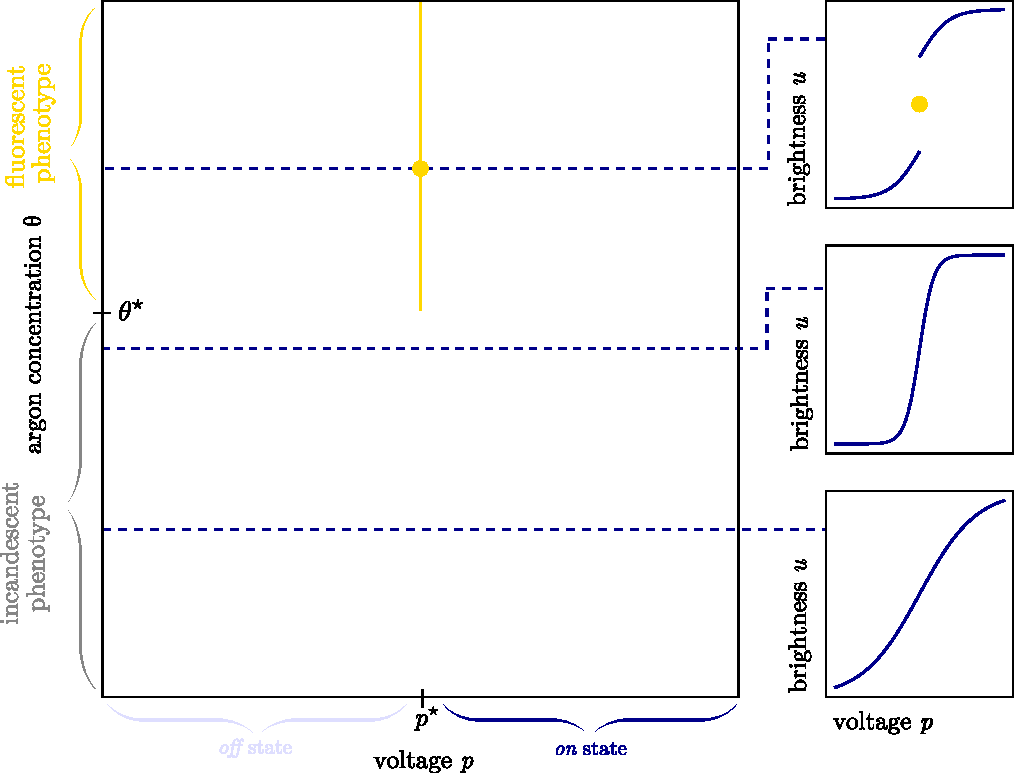
\includegraphics[scale=0.7]{bulb}
\caption{a) The bifurcations (shown in gold) at critical voltage $p^\star$ above argon concentration $\theta^\star$ give rise to sudden jumps in brightness (right-hand panels). $\theta^\star$ separates two bulb phenotypes and $p^\star$ separates the \emph{on} and \emph{off} states.}
\label{fig:bulb}
\end{Figure}

The fluorescent and incandescent bulbs can be considered as two different phenotypes distinguished by the quality of their response to voltage changes. Different colour bulbs can also be considered phenotypes, distinguished by the quality of their \emph{on} state, rather than their response to voltage. Bifurcation theory allows us to describe the transitions between qualitative states and can be leveraged to distinguish and organise phenotypes. In this context a bifurcation becomes a punctuation that either \emph{distinguishes between phenotypes} or \emph{distinguishes between behaviours within a phenotype}.

Suppose we inserted a component into our light bulb that changed parameter $\theta$ in such a way so that we can change between the discrete response of the fluorescent bulb and the continuous response of the incandescent bulb. Perhaps $\theta$ could be the concentration of argon gas; the bulb would have to be wired to behave like an incandescent bulb at low concentrations. We could collect brightness $u$ as a function of voltage $p$ and gas concentration $\theta$ produce something similar to that shown in Figure \ref{fig:bulb}. The bifurcations at critical voltage $p^\star$ above argon concentration $\theta^\star$ give rise to sudden jumps in brightness. The bifurcations separate the \emph{on} and \emph{off} states of the bulb and are only present in the fluorescent phenotype. The two phenotypes lie either side of  the onset of bifurcations at concentration $\theta^\star$. We can see from Figure \ref{fig:bulb} how knowing the locations of bifurcations allows us to organise qualitative behaviours and hence phenotypes of the bulb.

In the biological context, we can consider changes in $\theta$ as changes in the organism genotype that may or may not lead to a new phenotype. The idea of describing phenotypes in this way has been done before by Waddington \cite{}. His epigenetic landscape is a metaphor for how changes gene regulation, in our case represented by changes in $\theta$, determines the fate of cells. He imagines the cell as a marble, rolling down a series of forking valleys representing a differentiation cascade, eventually settling in its final phenotype. Let us adopt this metaphor for organism behaviours in response to a controlled condition (Figure \ref{fig:waddington}). Changing the control condition places the marble at different points in the valley and each fork in the valley corresponds to different available behaviours to the organism. Changing the parameters $\theta$ changes the topology of the valleys potentially giving rise to new behaviours and therefore new phenotypes. Due to the robustness \cite{} and fragility \cite{} of organisms we expect most changes in $\theta$ to either kill the organism or do nothing at all. The emerging picture suggests that the route between phenotypes is a carefully created sequence of changes in $\theta$.

\begin{Figure}
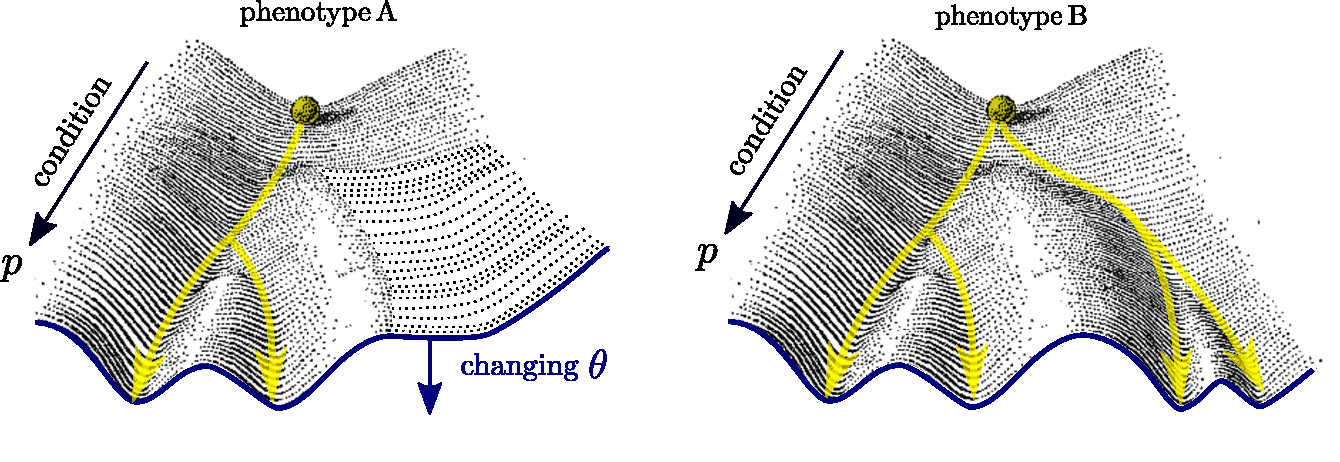
\includegraphics[scale=0.6]{waddington}
\caption{Waddington landscapes representing the set of available behaviours for two phenotypes in response to a controlled condition $p$. Phenotypes are related by changes in landscape topology via changes in $\theta$}
\label{fig:waddington}
\end{Figure}

In order to enumerate the phenotype distribution in the the high-dimensional parameter space $\theta$ for a given organism we must construct a model. By parametrising such a model $\rates(u,p)$ by $\theta$, we can relate the states of the organism $u$ to experimentally controlled conditions $p$. Ideally a subset of $u$ can be observed experimentally so that we may observe bifurcations in the data, as demonstrated in the right-hand panel of Figure \ref{fig:bulb}. In the following section we shall go through a class of models that can leverage bifurcation theory.  

% The problem is that the space of decisions that change $\theta$ is intractably large. Furthermore there is no guarantee that any two phenotypes would be connected via experimentally accessible changes in $\theta$. We will see in the incorporated publication in Chapter \ref{chapter:double-exclusive} how differential equation modelling and machine learning can be used to guide experiments and the genetic engineering of \emph{E. coli} towards a phenotype referred to as the \emph{double exclusive reporter}. 

% In the collaboration, bifurcation theory \cite{} was used to detect the onset of the desired phenotypic behaviour in a set of differential equations that model the engineered genetic circuits in \emph{E. coli}. We will see in the following sections how bifurcation theory is perfectly suited for modelling transitions between phenotypes, and hence popularised in fields such as synthetic biology and ecology. Through the use of machine learning and bifurcation theory in the same collaboration, we identified a gap: \emph{there existed no differentiable machine learning method that leveraged bifurcation theory directly}. The incorporated publication in Chapter \ref{chapter:inference} fills this gap, enabling an efficient exploration of phenotypes in the high-dimensional space of $\theta$.

% The antimicrobial resistance originates from selective pressures in the environment which change biochemical pathways which we can encode in parameters $\theta$. Neurons also have pathways that regulate aspects such as thickness of myelin sheaths on axons, that in turn dictate how sensitive, if at all, they are to firing. In the case of the \emph{Zebrafish} the parameters $\theta$ encode whether a particular mutation in the genome is present or not. 

% Synthetic biologists like to import such engineering metaphors when designing genetic sequences that would produce a desired behaviour. Genetic components are designed to be modular and mass produced like electrical components. with various behaviours are mass produced.

% This could be, for example, a phenotype of antimicrobial resistant bacteria \cite{Baym2016SpatiotemporalLandscapes}. We can break down this observation as follows: a cell can be in the qualitative state of \emph{resistant} or \emph{not resistant} at a certain concentration $p$ of antibiotic. Another example could be that of action potentials in neurons \cite{}. A neuron can either be \emph{firing} or \emph{not firing} in response to a given electro-chemical potential $p$. Whole organism phenotypes, such as pigment patterns \emph{Zebrafish} \cite{}, can also be described this way. In this case the phenotype emerges as the organism develops and therefore we look for emergence of \emph{patterns} or \emph{no patterns} over time $p=t$.

% In practice we can only observe a subset of the states, for example by incorporating fluorescent proteins downstream of the coding sequences of the proteins that participate in the antimicrobial resistance. Incorporating any fluorescent proteins into the host genome contributes to cell burdon and at worst can disrupt the mechanism under study. Therefore incorporation sites much be chosen sparsely such that the qualitative behaviour is still observable in the data.

\clearpage
\subsection{Differential Equation Models}

For the purposes of this thesis we will assume that the behaviour of the organism under study can be cast in terms of differential equations in a $N$ states $u$, $M$ parameters $\theta$ and $P$ control conditions $p$. For now we shall state the general class of models and follow up with concrete biological examples as we explore different types of bifurcations. Throughout the thesis we will consider models of the form

\begin{equation}
	\frac{du}{dt} = \rates(u,p)
	\where
	\begin{cases}
		\quad F: \Reals^{N+P}\rightarrow\Reals^N \\
		\quad \theta\in\Reals^M, u\in\Reals^N, p\in\Reals^P
	\end{cases}
	\label{eq:differential-equations}
\end{equation}

\noindent The total derivative $\frac{du}{dt}$ gives us the rate of change of the states with respect to time $t$ and all variables have been vectorised with the appropriate dimension. In principle the right-hand-side $\rates$ can be arbitrarily complicated, containing spatial derivatives or even machine learning models such as neural networks. We shall see later when such models become relevant in biomedical modelling.

\subsubsection{Trajectories \& Field Geometry}

In principle once equations \eqref{eq:differential-equations} have been written down they can be integrated to obtain trajectories $u(t)$ for various initial conditions $u(t')$. We can write the solution down formally as
\begin{equation}
	u(t) = u(t') + \int_{t'}^{t} \rates(u(s),p)\,\mathrm{d}s
	\label{eq:trajectory}
\end{equation}
Here the integral reveals that in order to determine where the state is at time $t$ we need to sum all the contributions of the function $\rates$ from the initial time $t'$ all the way up to final time $t$. The function $\rates$ depends on the state $u$ and must be updated with the integration variable $s$. This calculation can be interpreted, as shown in Figure \ref{fig:fields}, as choosing an initial point $u'=u(t')$ in a vector field $\rates$ and following the field lines until time $t$ at which the final point $u=u(t)$ has been reached.

\begin{Figure}
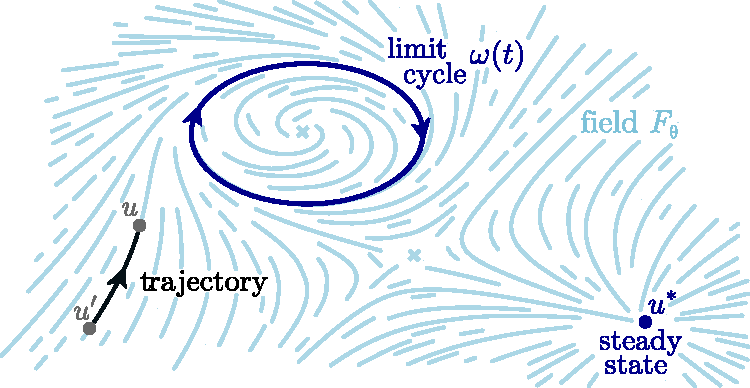
\includegraphics[scale=0.9]{fields}
\caption{Illustration of a trajectory between $u=u(t)$ and $u'=u(t')$ over finite time $t-t'$ following the field lines of $\rates$. In this example field lines either point towards steady state $\steady$ or a limit cycle $\cycle(t)$. There are two unstable fixed points marked by crosses: a saddle point separating the basins of attraction and an unstable focus enclosed by the limit cycle.}
\label{fig:fields}
\end{Figure}

By considering the geometry of the field $\rates$ in state space we can determine the fate of sets of trajectories, which are ultimately pulled towards \emph{dynamical attractors}. Such attractors can be static steady states $\steady$ or dynamic like the limit cycle $\cycle(t)$ illustrated in Figure \ref{fig:fields}. \emph{Dynamical attractors} create basins of attraction defined as regions of state space in which trajectories are pulled towards the same stable structure. These basins must be separated by unstable structures, such as the saddle point marked by a cross in Figure \ref{fig:fields}, which define a boundary between the basins called the separatrix. Note that the direction of the field $\rates$ and not its magnitude $|\rates|$ determines the fate of a trajectories.

When equations \eqref{eq:differential-equations} describe the behaviours of an organism, the attractors determine the set of qualitative behaviours available to the organism of genotype $\theta$, whilst experiencing experimental conditions $p$. If changes to the genotype $\theta$ change the number, type or stability of the attractors then we will observe new qualitative behaviours and hence a new phenotype. If changes to conditions $p$ lead to changes in the state space geometry, this is interpreted as a different behavioural state available to the same phenotype. We can see therefore how casting a biomedical problem into the language of differential equations, allows us to characterise phenotypic traits with the geometry of attractors in state space. 

\subsubsection{The Jacobian Matrix}

In order to quantify the geometry of a local patch of state space $u$ we can imagine $\rates$ as a velocity field of water and place a tiny blob of ink surrounding the location $u$. The so called Jacobian matrix $\jacobian$ of partial derivatives at the location $u$ transforms the basis vectors $\hat u(t)$ defining the blob over a short period of time $\Delta t$ as depicted in Figure \ref{fig:jacobian}. The transformation is
\begin{equation}
	\hat{u}(t+\Delta t)=\left (\mathbb{1}+\jacobian\Delta t \right)\hat{u}(t)
	\where
	\hat{u}\in\Reals^N\quad
	\jacobian\in\Reals^{N\times N}
	\label{eq:jacobian-transformation}
\end{equation}

\begin{Figure}
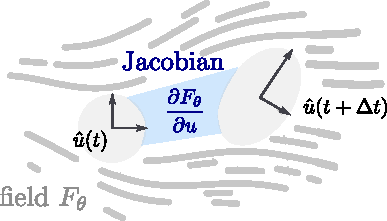
\includegraphics[scale=1.2]{jacobian}
\caption{Illustration how the Jacobian matrix $\jacobian$ transforms the basis vectors $\hat u(t)$ defining a small patch of initial conditions for a short period of time $\Delta t$. The eigenvalues $\lambda$ and eigenvectors $\eigenvector$ define the deformation of the patch}
\label{fig:jacobian}
\end{Figure}
\noindent where $\mathbb{1}$ is the identity matrix. The eigenvalues $\lambda$ and eigenvectors $\eigenvector$ of the Jacobian reveal to us the magnitudes and directions of the stretching or squeezing of the blob. We can diagonalise the Jacobian to obtain the eigenvalues and eigenvectors at any state space location $u$ to quantify the local geometry of the field. The eigenvalue equation is written as

\begin{equation}
	\lambda \eigenvector = \jacobian\eigenvector
	\where
	\eigenvector\in\Reals^N : |\eigenvector|=1
	\label{eq:jacobian-eigenproblem}
\end{equation}
where the eigenvectors are normalised to have unit magnitude. We can take the limit $\Delta t\rightarrow 0$ of equation \eqref{eq:jacobian-transformation} to obtain a first order matrix differential equation for the evolution of basis vectors $\hat u(t)$ in any patch $u$
\begin{equation}
	\frac{d\hat{u}}{dt}=\jacobian\hat{u}
	\label{eq:jacobian-odes}
\end{equation}
The coefficients given by the Jacobian matrix are time-independent and therefore the general solution can be written as a matrix exponential
\begin{equation}
	\hat{u}(t)=\e^{\jacobian(t-t')}\hat{u}(t')
	\label{eq:basis-vector-evolution}
\end{equation}
where $\hat{u}(t')$ are the basis vectors that define the initial shape of the blob centred on location $u$. If we let the basis for the initial blob be parallel to the eigenvectors $\eigenvector$ of the Jacobian, then the evolution any vector $\sigma(t)$ within the blob expressed in its basis becomes the linear superposition
\begin{equation}
	\sigma(t)= \sum_{\lambda}\eigenvector
	\sigma_{\lambda}(t') \e^{\lambda(t-t')}
	\label{eq:eigenbasis-vector-evolution}
\end{equation}
where $\sigma_{\lambda}(t')$ are the initial components of the vector in the basis of the blob. This equation reveals explicitly how the sign of real parts to eigenvalues $\Real\lambda$ determine the exponential growth or shrinkage of the blob in the direction $\eigenvector$. The imaginary parts $\Imag\lambda$ determine the magnitude of rotations of the blob. Note that since the Jacobian matrix is real and eigenvalues and eigenvectors appear in conjugate pairs and therefore the overall evolution \eqref{eq:eigenbasis-vector-evolution} yields real transformations of blob vectors $\sigma(t)$. The transformation \eqref{eq:jacobian-transformation} an approximation of the time-ordered exponential transformation \cite{} and we should note that the results stated here are valid for small blobs $|\sigma(t)|\ll 1$ over short timescales $|t-t'|\ll1$.

\subsubsection{Time Ordered Exponetials}

In this section we go a bit deeper into the origin of transformation \eqref{eq:jacobian-transformation} for those who are interested the evolution of state space blobs over arbitrary time intervals. We begin by considering the evolution of the separation between a trajectory $u(t)$ and its perturbation $u(t)+\delta u(t)$
\begin{equation}
	\frac{d}{dt}(u+\delta u) = \rates(u+\delta u,p)
\end{equation}
After Taylor expanding the field $\rates$ and recognising that equations \eqref{eq:differential-equations} lead to a cancellation in the terms involving the unperturbed trajectory $u$ we arrive at
\begin{equation}
	\frac{d}{dt}(\delta u) =
	\left.\jacobian\right|_{u=u(t)}\!\!\delta u + \mathcal{O}(\delta u^2)
	\label{eq:linearised-differential-equations}
\end{equation}
where $\jacobian$ is the Jacobian of the field and additional terms $\mathcal{O}(\delta u^2)$ involve taking higher order derivatives of the field $\rates$. Choosing a perturbation sufficiently small such that we can ignore higher order terms yields a first order homogenous ordinary matrix differential equation of the form $\dot{\delta u}(t)\approx J(t)\delta u(t)$ where $J(t)$ is a time-varying Jacobian. These equations can be solved formally with time-ordered matrix exponentiation \cite{} 

\begin{Figure}
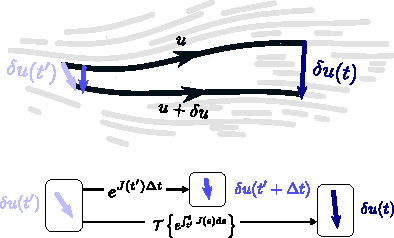
\includegraphics[scale=1.5]{lyapunov}
\caption{Illustration how the time ordering operator $\mathcal{T}\left\{\e^{\int_{t'}^t J(s) \mathrm{d}s}\right\}$ propagates the separation $\delta u(t)$ between adjacent trajectories $u$ and $u+\delta u$ by repeated application of the exponentiated Jacobian $\e^{J(t)\Delta t}$ evaluated along trajectory $u(t)$}
\label{fig:lyapunov}
\end{Figure}
\begin{equation}
	\delta u(t) \approx
	\mathcal{T}\left\{\e^{\int_{t'}^t J(s) \mathrm{d}s}\right\}\delta u(t')
	\where
	J(t) := \left.\jacobian\right|_{u=u(t)}
	\label{eq:matrix-exponential}
\end{equation}
The time-ordering defines an ordered product of matrix exponentials
\begin{equation}
	\mathcal{T}\left\{ \e^{\int_{t'}^t J(s) \mathrm{d}s} \right \}:=
	\lim_{\Delta t\rightarrow 0}\left(
		\e^{J(t)\Delta t}\e^{J(t-\Delta t)\Delta t}\,\dots\,
		\e^{J(t'+\Delta t)\Delta t}\e^{J(t')\Delta t}
	\right)
	\label{eq:time-ordering-operator}
\end{equation}
which can be calculated by repeated exponentiation of the Jacobian $\e^{J(t)\Delta t}$ evaluated at different times along the unperturbed trajectory $u(t)$. Although this expression may look complicated it is just another matrix whose eigenvalues reveal whether the trajectories diverge $|\delta u(t\rightarrow\infty)|\rightarrow\infty$ or converge $|\delta u(t\rightarrow\infty)|\rightarrow0$.

In situations where we want to investigate field flow over longer time intervals or where there is an explicit time dependence in the field $\rates(u,p,t)$ we must use the time-ordered exponential \eqref{eq:time-ordering-operator} in place of the exponentiated Jacobian.

\subsubsection{Lyapunov Exponents}
Sometimes we are only interested in the rate of change of the magnitude of deformations $|\sigma(t)|$ which can quantified by the \emph{finite time lyapunov exponent}
\begin{equation}
	\Lambda(u,\Delta t):=\frac{1}{\Delta t}\log\frac{|\sigma(t+\Delta t)|}{|\sigma(t)|}
\end{equation}
We remind ourselves that the blob $\sigma(t)$ is centred around state space point $u$, then evolved for a time $\Delta t$ and therefore the exponent is a function of $\Delta t$ and $u$. Substituting equation \eqref{eq:eigenbasis-vector-evolution} we arrive at
\begin{equation}
	\Lambda(u,\Delta t) = \frac{1}{2\Delta t}\log
	\left\langle
		\e^{2\Real[\lambda]\Delta t}
	\right\rangle_{\sigma(t)}
	\ge 
	\left\langle
		\Real[\lambda]
	\right\rangle_{\sigma(t)}
	\label{eq:finite-time-lyapunov}
\end{equation}
where $\left\langle\cdots\right\rangle_{\sigma(t)}$ is a shorthand for a weighted arithmetic average over the components of the initial blob $\sigma(t)$. We have used Jensen's Inequality \cite{} to show that the rate of distortions is bounded by the average of real parts of eigenvalues. This bound becomes an equality for eigenvalue $\lambda$ when the blob $\sigma(t)$ is initialised along only its eigenvector $\eigenvector$. We will see later how the \emph{Lyapunov exponents} are useful for extracting timescales around interesting structures in state space such as \emph{fixed points} and \emph{degeneracies}. 

\subsubsection{Fixed Points}

Thusfar we explored the field geometry in arbitrary patches of state space $u$ and asked questions about local flows. It is usually not possible to set up experimental conditions to get an organism to trace out all of its available states without killing it or distorting the mechanism under study. An organisms prefers to operate within a finite set of states and would want to return to them when perturbed. This is a hallmark of a stable steady state $\steady$ which belongs to a wider class of points called \emph{fixed points}. In the context of differential equation models, a \emph{fixed point} is the solution of
\begin{equation}
	\left.\frac{du}{dt}\right|_{u=\steady}=\rates(\steady,p) = 0
	\label{eq:fixed-point-equation}
\end{equation}

\begin{Figure}
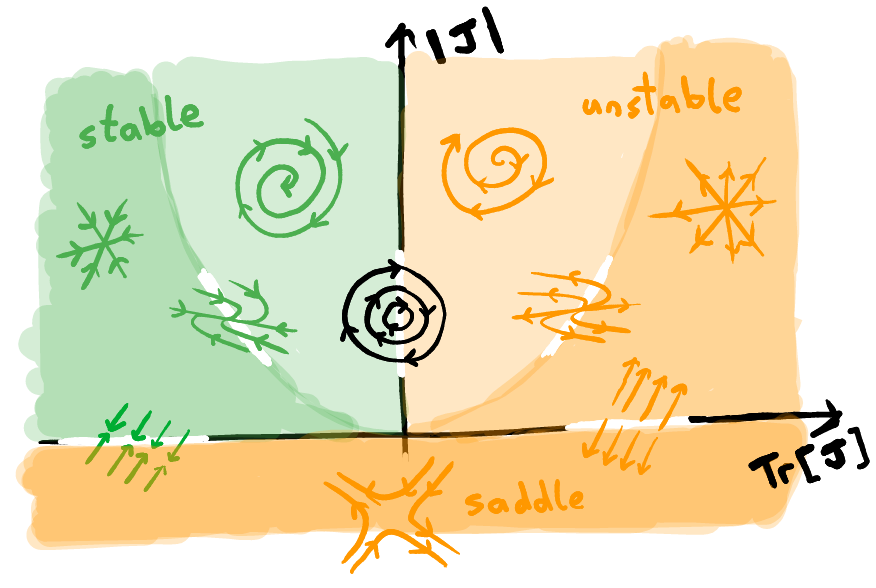
\includegraphics[scale=0.35]{stability}
\caption{Classification of stable and unstable fixed points for a general two dimensional systems in terms of trace $\mathrm{Tr}[\jacobian]$ and determinant $|\jacobian|$ of its Jacobian}
\label{fig:stability}
\end{Figure}

By looking at the eigenvalues of the Jacobian, which determine local flows according to equations \eqref{eq:eigenbasis-vector-evolution}, we can classify the fixed point $\steady$. The sign of real parts $\Real\lambda$ determine whether small perturbations away from the fixed point will diverge. This defines whether the point is \emph{stable}, \emph{unstable} or a \emph{saddle}. Non-zero imaginary parts $\Imag\lambda \ne 0$ give rise to damped oscillation around the point; these points are called \emph{foci}. Without real parts the flow becomes purely rotational and give rise to \emph{cycles}.

For a two dimensional system we can express the two eigenvalues of the $2\times 2$ Jacobian in terms of its trace $\mathrm{Tr}[\jacobian]$ and determinant $|\jacobian|$ which allows us to conveniently reveal all the possible fixed points types, as in Figure \ref{fig:stability}. If at least one the eigenvalues vanishes the fixed point becomes \emph{degenerate}. We shall see that \emph{degenerate} field flows lead to critical slowing down in dynamics, reveal bifurcations and are useful for constructing tangent fields to implicitly defined surfaces.

\subsubsection{Field Degeneracy}
A field $\rates$ can be called \emph{degenerate} where it is locally constant and hence does not cause shape changes to a blob of initial conditions in one or more directions. This means that one or more of the eigenvalues of the Jacobian vanish $\lambda = 0$ and have associated eigenvectors $\hat T_\lambda$ tangent to the direction where the field is locally constant. Suppose the field is \emph{degenerate} at point $\degenerate$, then the vanishing eigenvalues lead to a zero determinant $\left|\jacobian\right|=0$ and the eigenvectors must be orthogonal to all the gradients
\begin{equation}
	\left|\jacobian\right|_{u=\degenerate} \!\!\! = 0
	\qquad\left.\jacobian\right|_{u=\degenerate}\!\!\!\hat T_\lambda = 0
	\where
	\hat T_\lambda\in\Reals^N : |\hat T_\lambda|=1
	\label{eq:degeneracy-conditions}
\end{equation}
The eigenvector equation yields $\hat T_\lambda$ that span the degenerate subspace at field location $\degenerate$. The number of vectors and hence the size of the subspace is given to us by the number of vanishing eigenvalues $\lambda=0$. In linear algebra this would be referred to as the \emph{nullspace} or \emph{kernel} of the Jacobian matrix. A vanishing determinant means that the Jacobian is not invertible.

\subsubsection{Critical Slowing Down}
% A fixed point $\steady$ that is also degenerate $\degenerate$ is called a critical point $\critical$. This is a location in the state space that satisfies equations \eqref{eq:fixed-point-equation} and \eqref{eq:degeneracy-conditions}. This means that the field $\rates$ is not only zero, but also locally zero along at least one direction. In this case the whole degenerate subspace takes on the character of the fixed point and gives rise to power law timescales that are characterised using \emph{critical exponents}.

% \emph{Critical exponents} are not the same as \emph{Lyapunov exponents} although we will see that they are related. These exponents are important because the power laws can be detected in trajectory data and can be used to classify bifurcations.

Lets us consider the magnitude of deformations along the degenerate direction $T_\lambda(t)$ in the vicinity of the the region $u\approx\degenerate$ that is driven by the scalar sub-field $F_\lambda$. We expect the first-order derivatives to vanish $\left.\frac{dF_\lambda}{dT_{\lambda}}\right|_{u=\degenerate}\!\!\!\!\!\!\!\!\!\!\!\!\!\!\!=0$ and therefore have to expand the field $F_\lambda$ to an order $n$ that will yield the first non-zero derivative. The equations expanded for $u\approx\degenerate$ are
\begin{align}
	\frac{d T_\lambda}{dt} &= \left.\frac{dF_\lambda}{dT_{\lambda}}\right|_{u\approx\degenerate}
	\!\!\!\!\!\!\!\!\!\!\!\!T_\lambda(t) +
	\frac{1}{n!}
	\left.\frac{d^n F_\lambda}{dT_{\lambda}^n}\right|_{u\approx\degenerate}
	\!\!\!\!\!\!\!\!\!\!\!\!T_{\lambda}(t)^n +\mathcal{O}(T^{n+1})
	\where n \ge 2
	\label{eq:bernoulli-differential-equation}
\end{align}
Here we kept the first-order derivative because we would still like to see how the dynamics scales with time as we approach to degeneracy. This is a Bernoulli differential equation \cite{} with constant coefficients and has a general solution
\begin{align}\!\!\!\!\!
	T_{\lambda}(t) = \left(
	\left(T_{\lambda}(t')\e^{(t-t')
	\left.\frac{dF_\lambda}{dT_{\lambda}}\right|_{u\approx\degenerate}
	}\right)^{1-n}
	-(t-t')\frac{n-1}{n!}\left.\frac{d^n F_\lambda}{dT_{\lambda}^n}\right|_{u\approx\degenerate}
	\right)^{\frac{1}{1-n}}
	\label{eq:critical-slowing}
\end{align}

This equation reveals two timescales for blob deformations in the vicinity of a field degeneracy: the familiar exponential timescale $\e^{t-t'}$ and a new polynomial timescale $(t-t')^{\frac{1}{1-n}}$. The emergence of a polynomial timescale that dominates over the exponential is called \emph{critical slowing down} and is a marker of degeneracy. We can see once the dynamics is confined to the degenerate subspace the eigenvalues of the Jacobian are insufficient for determining the timescales. The curvature of the field around the degenerate subspace drives the polynomial dynamics, and therefore higher-order derivatives are needed to reveal this.

This critical slowing can be observed in data when \emph{fixed points} become \emph{degenerate}. Degenerate fixed points are also called \emph{critical points}. The transition between these two timescales in data is a signal that a \emph{critical point} is nearby. We will see that \emph{critical points} may lead to bifurcations and bifurcations are always accompanied by degeneracies in the field.

\subsubsection{Limit Cycle Analysis}
Thusfar we dealt with static state space structures like \emph{fixed points}. We found that the eigenvalues of the Jacobian are sufficient for their characterisation, unless the field is  \emph{degenerate}, in which case higher order derivatives of the field must be investigated.

If fields lines point towards a region of state space but the region \emph{does not} contain any fixed points, then the only other option is for the field lines to converge onto a \emph{limit cycle}. This is actually a rough statement of the Poincar\'e-Bendixson theorem  which allows us to define trapping regions where trajectories do not escape from and make statements about the existence or non-existence of limit cycles. A limit cycle must also enclose a finite number of \emph{unstable foci} that push trajectories away from its center.

Newton-type methods can easily be applied to find \emph{fixed points} because they are local structures in fields. Limit cycles are much more tricky because it is not possible to know whether a local state part of a limit cycle or not before we have seen a trajectory visit that state twice: once at $u(t)$ and then again $u(t+T)$ after some time $T$. This forms the basis of some optimisation methods for computing limit cycles \cite{}.

\begin{itemize}
	\item Trapezoid method
	\item Collocation method
	\item Shooting method
\end{itemize}

% \begin{Figure}
% 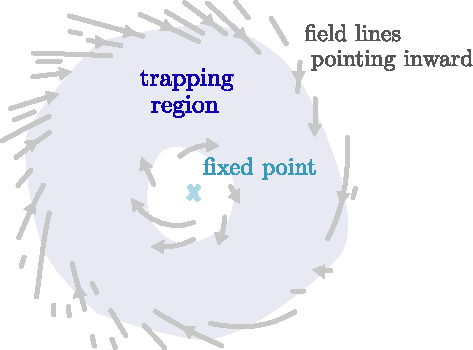
\includegraphics[scale=0.35]{limit-cycle}
% \caption{}
% \label{fig:limit-cycle}
% \end{Figure}

\clearpage
\subsection{Bifurcation Analysis}
\label{section:bifurcation-analysis}
We have surveyed sufficiently many state space structures, the geometry of which determine the qualitative behaviour of the organism we are describing. An organism has many qualitative behaviours in response to conditions $p$ and many phenotypes emerging from changes in $\theta$.

Bifurcations are defined as qualitative changes to system behaviour in response to smooth changes to some conditions. In our setting these conditions could be either $\theta$ or $p$, but we will focus on changes with respect to $p$ with the understanding that the analysis is equally valid for $\theta$. We are ready to present the two \emph{generic} and \emph{robust} one parameter bifurcations: the \emph{saddle-node} and \emph{Hopf} bifurcation. These bifurcations are generic in the sense that they happen in $N$ dimensional systems, but can be described as happening along one dimension. This is true because of centre manifold theory \cite{}. The bifurcations are \emph{robust} in the sense that small changes to system parameters do not destroy the bifurcation. This is not the case for \emph{pitchfork} and \emph{transcritical} bifurcations which we will present in a separate section.
\subsubsection{Generic Robust Bifurcations}
\begin{Figure}
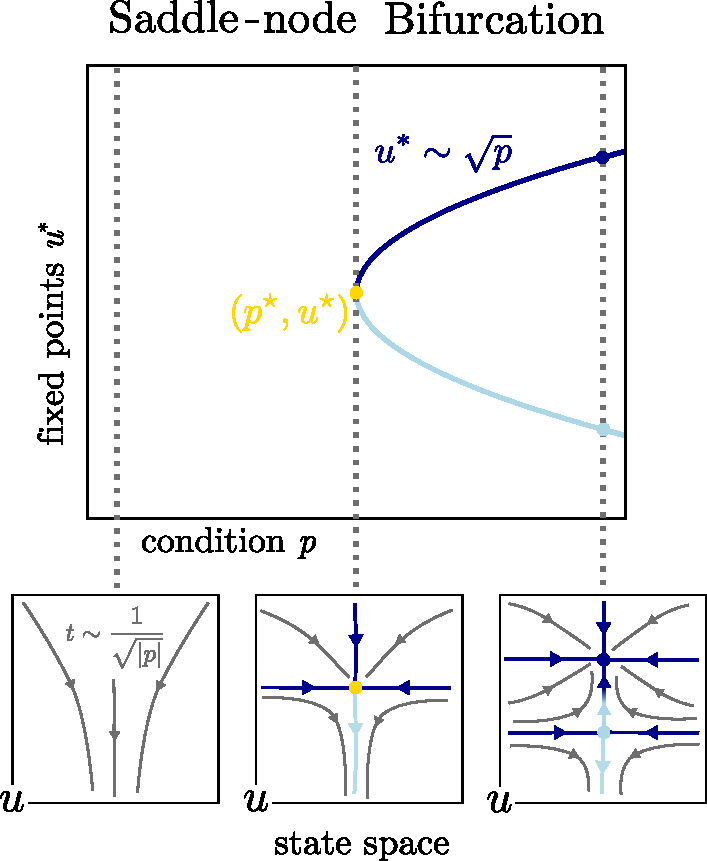
\includegraphics[scale=0.6]{saddle-node} 
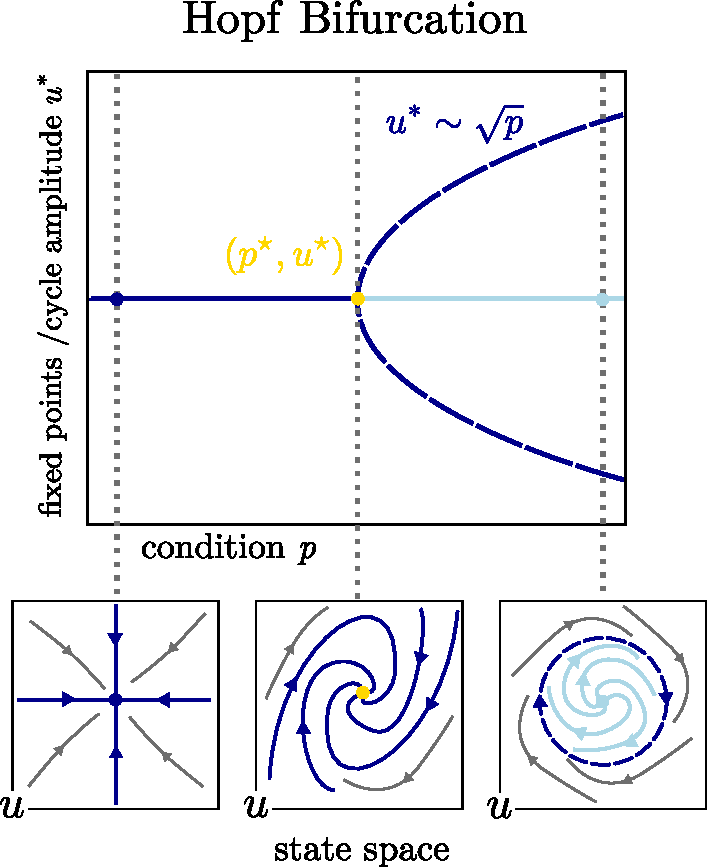
\includegraphics[scale=0.6]{hopf}
\caption{Generic and robust bifurcations. A. \emph{Saddle-node} bifurcations create or annihilate stable and unstable pairs of fixed points. B. In \emph{Hopf} bifurcations a stable fixed point becomes an unstable focus that pushes trajectories towards a limit cycle.}
\label{fig:robust-local-bifurcations}
\end{Figure}
\subsubsection{Fragile Bifurcations}
\begin{Figure}
	\begin{center}
	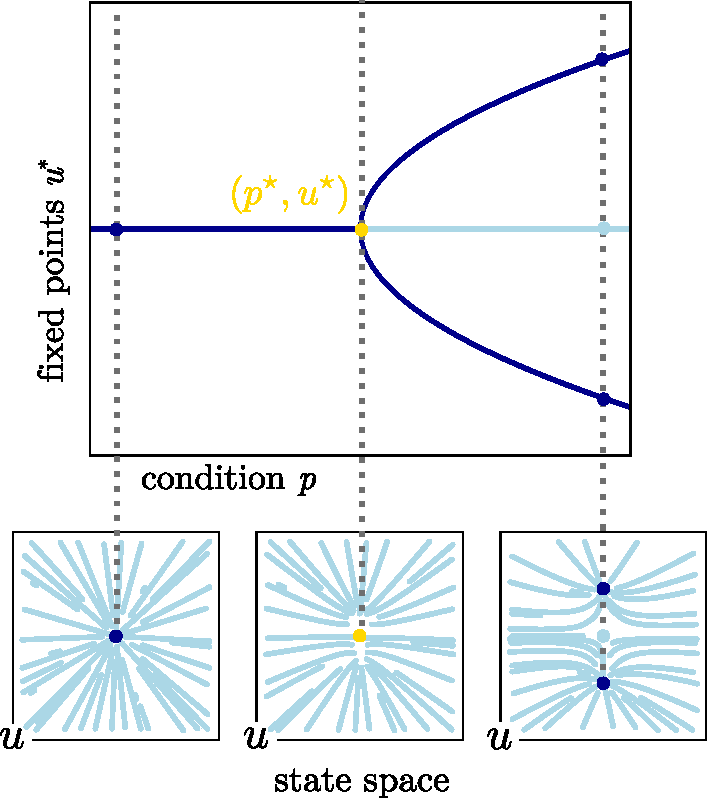
\includegraphics[scale=0.6]{pitchfork}
	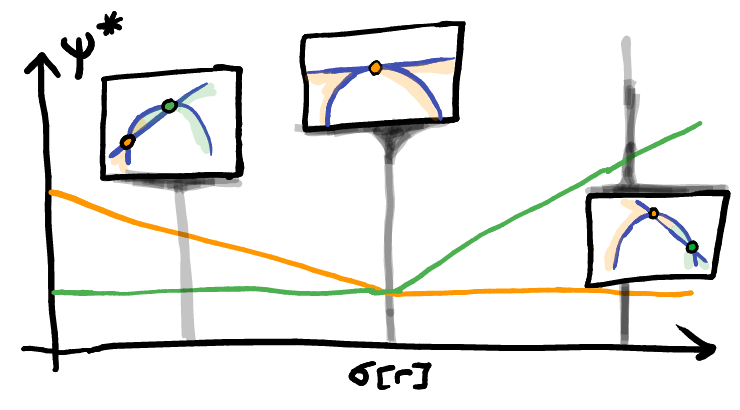
\includegraphics[scale=0.6]{transcritical}
	\end{center}
	\caption{Fragile bifurcations}
	\label{fig:fragile-bifurcations}
\end{Figure}
\subsubsection{Global Bifurcations}
\begin{Figure}
	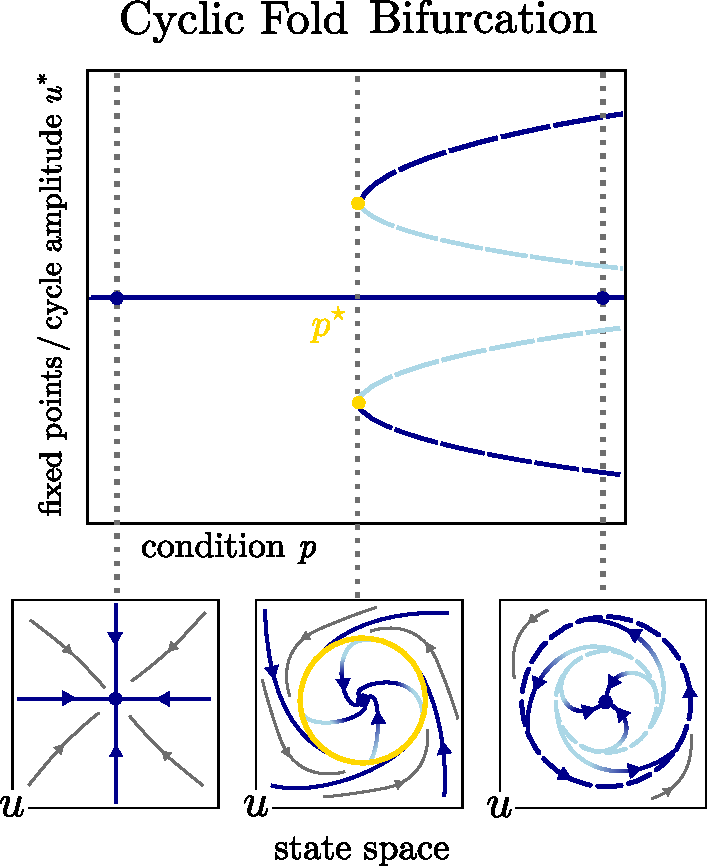
\includegraphics[scale=0.6]{cyclic-fold}
	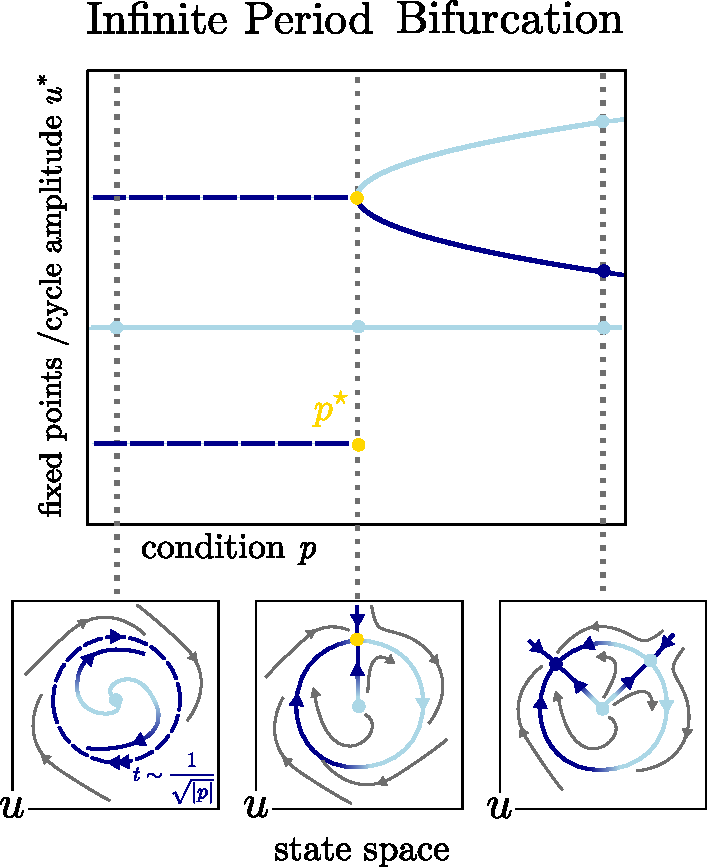
\includegraphics[scale=0.6]{infinite-period}
	\caption{Global Bifurcations}
	\label{fig:global-bifurcations}
\end{Figure}

\begin{Figure}
	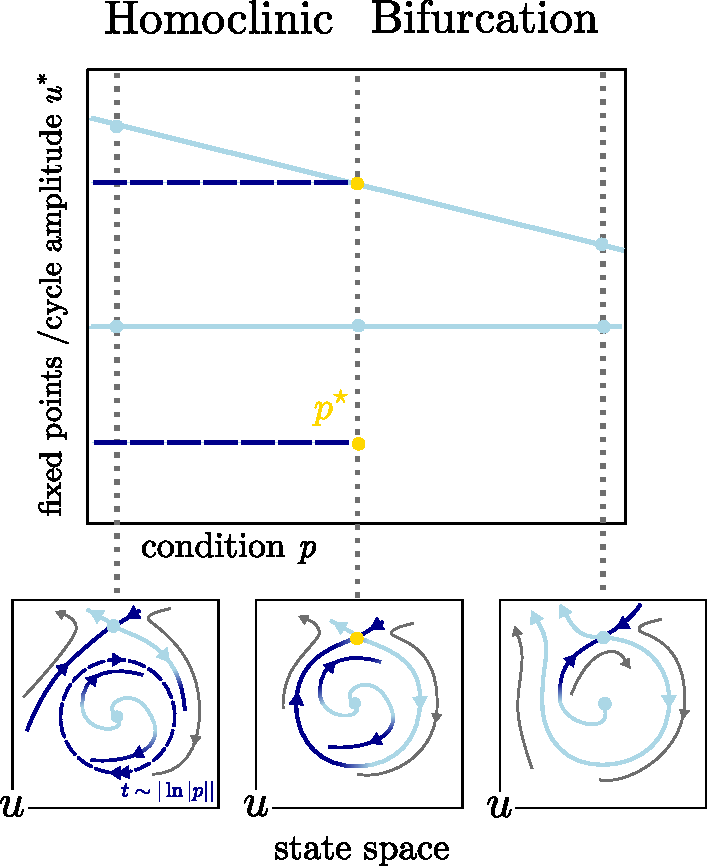
\includegraphics[scale=0.6]{homoclinic}
	\caption{Global Bifurcations}
	\label{fig:global-bifurcations}
\end{Figure}

\subsubsection{Higher Co-dimension}

\subsubsection{Parameter Continuation}

\subsection{Spatially Extended Systems}

If $\rates$ contains spatial derivatives, additional conditions on $u$ with respect to spatial variables $x\in\Reals^D$, where $D$ is the dimension of the space considered, must be supplied to give a unique solution $u(x,t)$.



\subsubsection{Turing Bifurcations}
When studying spatio-temporal dynamics of organisms, a popular choice is to incorporate a diffusive term that models the exchange of matter between spatial locations
\begin{align}
	\partial_t
	\psi &=
	\mathbf{\Gamma}\omega(\psi|\mathbf{\Gamma})
	\label{eq:reaction}
\end{align}


A bifurcation diagram tracks changes in attractors such as fixed points $\steady$ and limit cycles $\cycle(t)$ in response to changes in control conditions $p$.  In the next section we will see how fixed points and limit cycles are characterised with linear stability analysis

this can be done using 
In this thesis we extensively use the library \texttt{DifferentialEquations.jl} \cite{Rackauckas2017Differentialequations.jlJulia} for numerically solving differential equations and \texttt{BifurcationKit.jl} \cite{Veltz2020BifurcationKit.jl} for calculating bifurcation diagrams. 

Partial observation can be modelled explicitly with latent variables \cite{} or the explicit modelling of system and measurement device as is done in control theory \cite{}. For the scope of this thesis we will let the modeller have complete freedom on how to choose relevant state variables $u\in\Reals^N$ and write down their own set of differential equations, with unknown parameters $\theta\in\Reals^M$ of the form

\section{Applications in Cell Biology}
\label{section:applications-cell-biology}

\subsection{Genetic Switches \& Phenotype Boundaries}
These equations can originate from mean-field approximations of the chemical master equation \cite{} representing biochemical reaction networks \cite{}. This typically yields models with a large number of parameters $M$ and states $N$. The equations could have also undergone a series of quasi-steady state approximations \cite{} yielding hill-functions. Various other model reduction methods exist \cite{} in an attempt to reduce the number of state variables $N$ and parameters $M$.

\subsection{Populations of Neurons}

\subsubsection{Neural Differential Equations \& Gaussian Processes}
While principled derivation from microscopic rules exist, often the the number of variables $N$ participating in the mechanism under study becomes intractable. When the desire for predictive performance out-weighs the desire for mechanistic explanations, the states $u$ are chosen to be the observable subset for which we have data, and the right-hand side $\rates$ can be a machine learning model such as a neural network or Gaussian process \cite{}. In this case the number of parameters becomes much larger than the number of states $M\gg N$. A recent breakthrough in back-propagation through differential equation solvers \cite{} has made these models tractable in optimisation routines, and popularised them in literature \cite{}.


\subsubsection{Stochastic Differential Equations}


\subsection{Self-organised Patterns \& Development}

In this section we would explore the geometrisation of phase space, lyapunov
exponents and universality. Perhaps a discussion on phase transitions and
the relation to Landau-Ginzberg approaches is required.
Maybe also periodic orbit theory? Depends how useful it is.
\subsubsection{Reaction-Diffusion}
Here we first introduce diffusion macroscopically by simply adding the laplacian
to mean field equation $\eqref{eq:reaction}$. We introduce the turning bifurcation and
show how linear stability analysis is insufficient to capture pattern formation
and rich inhomogeneous steady states. A promising approach may be geometrisation
of the moving local equilibria \cite{Halatek2018}.

\section{Phenotype Inference with Machine Learning}
\label{section:phenotype-inference}
\begin{itemize}
    \item Preface on SciML community and gray-box modelling
\end{itemize}

\subsection{Classification and Regression}
\begin{itemize}
    \item Logistic regression
    \item Nearest neighbour methods
    \item Mixture Models
\end{itemize}

\subsection{Dimensionality Reduction Methods}
\begin{itemize}
    \item UMAP and Tsne
    \item Sloppy parameters and identify-ability
\end{itemize}

\subsection{Clustering Methods}

\section{Applications in Flow Cytometry}
\label{section:applications-flow-cytometry}


\subsection{Immunophenotyping Panels}


\subsection{Inferring Bifurcations from Data}

In sections \ref{inference:abstract} -- \ref{inference:impact} we assume that the bifurcation data $\targets$ with respect to the experimental control condition $p\in\Reals$ is known or already extracted from raw data. We can break down the extraction process into steps: steady state inference, field inference and fixed-point inference; each discussed separately in its own subsection. These steps are sequenced together into two possible routes towards bifurcation data $\targets$ as depicted in Figure \ref{fig:inferring-bifurcations}.

At best we could have state trajectory data like single cell trajectories extracted via segmentation and tracking in fluorescence microscopy movies (for example the data acquired using the CellASIC platform in Figure \ref{fig:double-exclusive:bistability}c). Having the the state as a function of time $u(t)$, sampled at sufficiently broad initial conditions $u(0)$, enables the \emph{non-parametric} estimation of field geometry $F(u)$. We can then extract important state-space structures, such as stable and unstable fixed points, their eigenvalues $\lambda$, from the field geometry $F(u)$ at different values of the control condition $p$, and hence identify possible bifurcations.

\begin{Figure}
    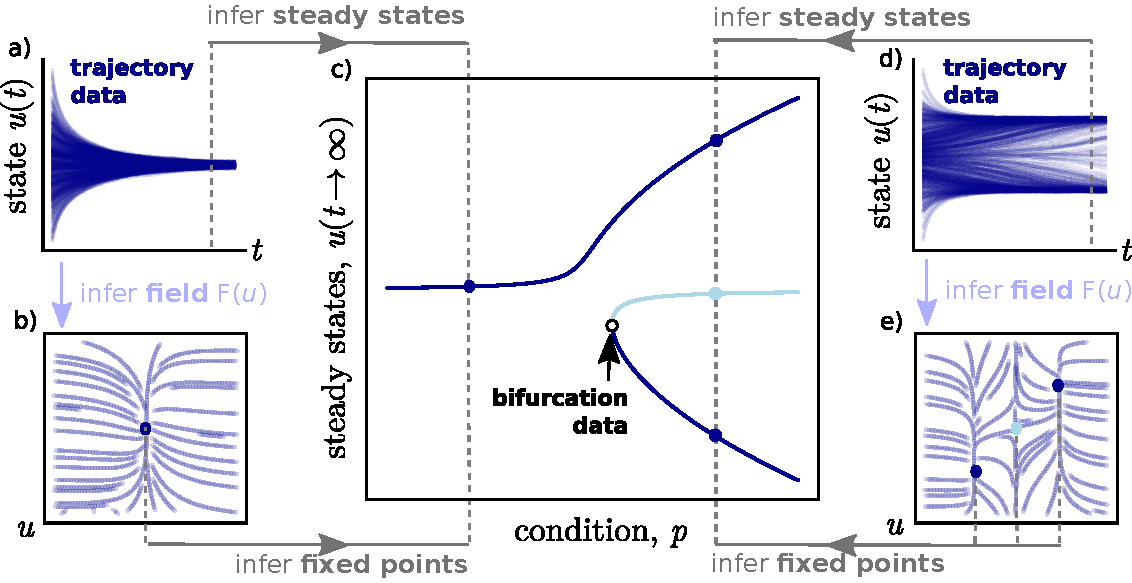
\includegraphics[width=14cm]{inferring-bifurcations}
    \caption{Bifurcation point extraction along the condition $p$ via two possible routes: steady state inference (a,d$\rightarrow$c) and fixed point inference (a,d$\rightarrow$b,e$\rightarrow$c). The fixed point inference route requires the geometry of the field $F(u)$ at different values of the condition $p$ and yields additional information about unstable fixed points.}
    \label{fig:inferring-bifurcations}
\end{Figure}
Data on steady states $u(t\rightarrow\infty)$ are more abundant and typically found in flow cytometry measurements. It is possible to infer the steady state manifold directly from such data (Figure \ref{fig:inferring-bifurcations} a,d$\rightarrow$c) but we would not be able to extract information on unstable fixed points or eigenvalues $\lambda$ of state-space structures. Since the criteria for bifurcations are not directly accessible, indirect measures (such as the population separation that can be seen in Figure \ref{fig:double-exclusive:flow-hysteresis}) must be used to extract bifurcations.

\subsubsection{Bifurcations via Steady State Inference}
\label{section:steady-state-inference}

Suppose we would like to detect a cusp bifurcation and limit points in a cell population with respect to two experimental control conditions $p,p\prime\in\Reals$. We can set up a serial dilution along the columns for $p$ and along the rows for $p\prime$ in two 96-well plates. Cells allowed to grow in exponential phase in a finite concentration of either $p\ll p\prime$ or $p\gg p\prime$. Let us call this the \emph{priming} stage of the protocol as shown in Figure \ref{fig:cusp-sampling}a, resulting in two cell populations: $p$-primed cells and $p\prime$-primed cells. The priming concentrations must be chosen sufficiently high so that the resultant population states lie either side of the cusp. The two populations are transferred into separate 96-well plates containing the dilutions of $p,p'$; we call this the \emph{conditioning} stage in Figure \ref{fig:cusp-sampling}a.

\begin{Figure}
    \includegraphics[width=14cm]{hysteresis}
    \caption{Protocols (a) for extracting limit points with respect to conditions $p,p'$. Steady state distributions (b). Similarity measure (c)}
    \label{fig:cusp-sampling}
\end{Figure}

The cells are then transferred into a flow cytometer, gated for live singlets and processed with relevant compensation and auto-fluorescent normalisation, which would produce the population distributions $P(u)$ for the $p$-primed cells and $Q(u)$ for $p'$-primed cells in each well. By overlaying distributions $P(u),Q(u)$ for each well, a figure similar to Figure \ref{fig:cusp-sampling}b (or Figure \ref{fig:double-exclusive:flow-hysteresis}) can be produced. Finally, the limit points can be defined by a level set of distribution similarity measure $D(P||Q)$ in the $p,p\prime$-plane as shown in Figure \ref{fig:cusp-sampling}c. This similarity measure could be Kullback–Leibler divergence or something as simple as the distance between distribution medians. The level set must be some small positive amount $\epsilon$ above zero, picking out the onset of dissimilarity between steady state distributions $P(u)$ and $Q(u)$, and hence the onset hysteresis. We can define the limit points as
\begin{align}
    \targets = \{  (p,p\prime) : D(P||Q)=\epsilon, \epsilon>0 \} 
\end{align}

This approach may break down if multi-modal distributions exist in the data. This would be the case if something happened to prevent a subpopulation of cells to switch from one state another other. Reasons for this could include too much cell burdon or not enough time given for cells to reach a steady state. In this case, quantifying the efficiency of switching from either side of the cusp could be a quantity of interest.

This approach would not work for extracting dynamic bifurcations such as \emph{Hopf} since only steady state information is available. Furthermore, the accuracy of this method is subject to noise amplitude. This method works well for cases where changes in the number of stable steady states can be resolved in the measured steady state distributions.

\begin{itemize}
    \item \todo[inline]{quantify efficiency of switching?}
\end{itemize}


\subsubsection{Non-parameteric Vector Field Inference}
% Non-parametric ___ using Gaussian Process regression
\label{section:field-inference}

In this early days of this thesis, we investigated whether it was possible to transform the time-domain data into state-space. This approach, and related works, are discussed in this section and can in principle be used with the microfluidic fluorescence microscopy data for parameter inference.

Consider we are given $K$ cell trajectories $\mathcal{D}_1$, $\mathcal{D}_2$ ... $\mathcal{D}_K$, each containing $N$ noisy observations of the state of the cell. Let the cell state be represented by state vector $u(t)\in\Reals^N$ which is hypothesized to obey a set of ordinary differential equations of the form \eqref{eq:differential-equations}. Instead of integrating the equations \eqref{eq:differential-equations} we would find an estimate for the derivative of the trajectories $\hat{f}$.

This is known as the \textit{smoothing} step \cite{Gugushvili2012Smoothing} should be done using unsupervised methods, for example with Gaussian Process Regressors \cite{Seeger2004GaussianLearning.} as shown in in Figure \ref{fig:inferred-cycles}. This requires the inversion of an $K'\times K'$ data matrix where $K':=\sum_k |\mathcal{D}_k|$ is the total number of trajectory data points. This has a computational complexity $K'^3$ which is only tractable with sparse datasets.

Let the region $\partial\mathcal{D}$ be a boundary defined by the Delaunay tessellation of the input data. Let us define the estimate $\hat f$ only within the region $\partial\mathcal{D}$ so that there are no extrapolation artefacts. For the Gaussian Process approach the estimate would be
\begin{equation}
    \hat{f}(u)\sim
        \mathcal{N}(\,\mu(u) ,\Matrix{\Sigma}(u)\,)
    \quad\mathrm{for}\quad u\in\partial\mathcal{D}
\end{equation}
\noindent where at any given state $u$ the field estimate $\hat{f}$ is generated by Gaussian distributions of mean vector $\mu$ and covariance matrix $\Matrix{\Sigma}$.Solving for these requires a choice of matrix-valued kernel function $\Matrix{K}(u,v)$ which encodes our knowledge about the local structure of the field. Sophisticated kernels for learning vector fields exist \cite{Fuselier2017ADecompositions} for decomposing fields in conservative and solenoidal components, which aid in localising fixed points and cycles.

The simplest choice of kernel assumes the components are independent and have a finite correlation length $\gamma$, such as Gaussian radial basis functions. Here $\Matrix{I}$ is the identity matrix and the hyperparameter $\gamma$ has to be optimised.
\begin{equation}
    \Matrix{K}(\Vector{u},\Vector{v}) = \Matrix{I}\,\mathbb{e}^{-\gamma|\Vector{u}-\Vector{v}|^2}
\end{equation}

The second step is called \textit{matching} where the estimated field $\hat{f}$ is used as an optimisation target against some parametrised function $\rates$ with unknown parameters $\theta$.

In our setting we would like to match the geometry of the field but not its magnitude; in this sense we are focusing on the qualitative aspects of the dynamics of a set of differential equations, rather than the quantitative dynamics or kinetics. This could be achieved with the following objective function
\begin{equation}
    \mathcal{L}(\theta|\mathcal{D}) := \e^{-\frac{\hat{f}\cdot\rates}
    {|\hat{f}||\rates|}}
\end{equation}
\noindent where the cost is minimal when the data derivative $\hat{f}$ and the parametrised model $\rates$ point in the same direction and maximal when they point in opposing directions.

\begin{Figure}
    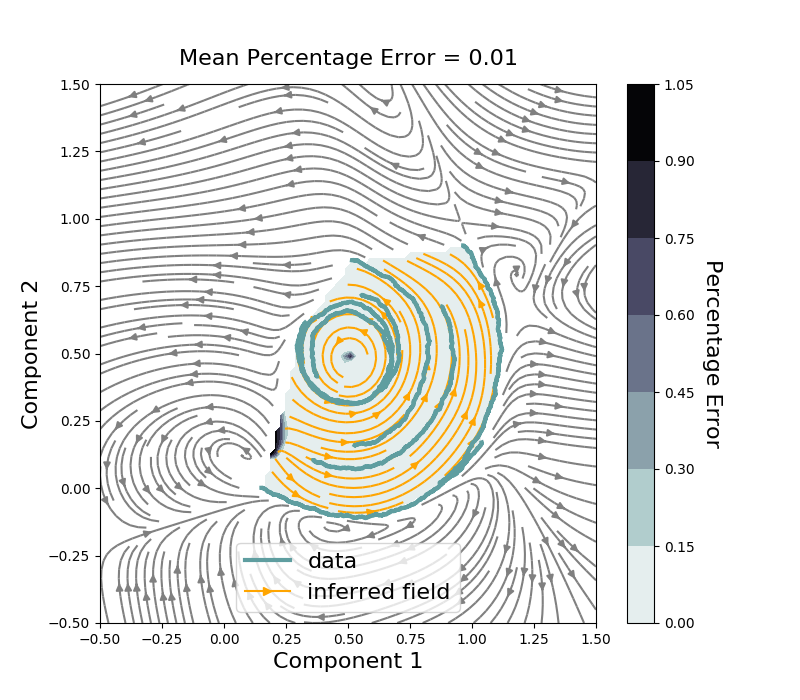
\includegraphics[width=125mm]{figures/cycle-2.png}
    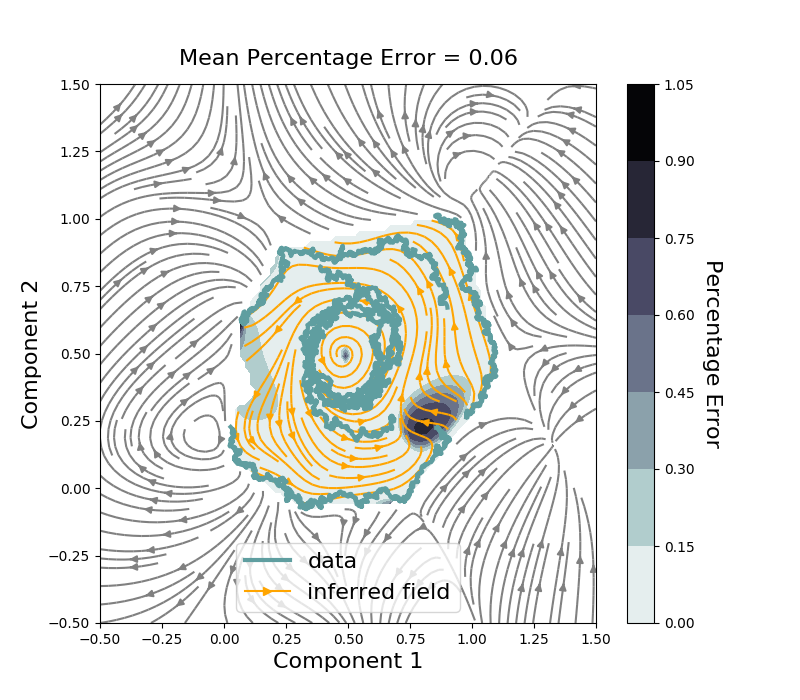
\includegraphics[width=125mm]{figures/cycle-1.png}
    \caption{Gaussian process regressors estimating derivative of the trajectories $\hat{f}$ from example trajectory datasets $\mathcal{D}_1$ ... $\mathcal{D}_K$ with varying signal to noise ratios. Interpolation error $E$ is shown as a heatmap; extrapolation fails}
    \label{fig:inferred-cycles}
\end{Figure}

Although we are getting close to focusing on qualitative features of a model, this objective function is still sensitive to the locations and shapes of fixed point and limit cycles. What if we cared about even higher-level features such as the number of fixed points? Or perhaps whether a system oscillates or not? This is where the language of bifurcation theory described in Chapter \ref{chapter:background} is optimally suited for this task, but fist we need to discuss how to set up experiments to detect bifurcations from flow cytometry data.

\begin{itemize}
    \item \todo[inline]{Vector field estimates too noisy to get bifurcation points?}
    \item \todo[inline]{Divergence and the stability of fixed points}
    \item \todo[inline]{Curl and limit cycles. How does this relate to hopf example \ref{fig:inferred-cycles}}
    \item \todo[inline]{Do we need a bistable example?}
\end{itemize}

The accuracy of the cell trajectories is limited by cell segmentation and tracking algorithms. Initial investigations into this approach also suggested that trajectories need to be of sufficient temporal resolution and sampled from a wide variety of initial conditions. Such data is not widely available and ultimately we decided to focus on a method that could be used with a well-known workhorse in biomedical research: flow cytometry.

\subsubsection{Fixed Point Inference}
\label{section:fixed-point-inference}